\chapter{Literature Review}
For the purpose of this project, an extensive investigation and comparative study into recently released Large Language Models has been conducted. This chapter delves into a comprehensive exploration of Text-Generative AI in general: it examines the concept and diverse applications of generative AI and a Retrieval-augmented Generation pipeline system, its elements and components alongside a comparison between their technical aspects, and its eventual limitations.
\newpage

\section{Text Generative AI}
The term Text Generative AI refers to the artificial-generation of textual content, it can allude to the tasks of next word suggestion, summarization, rewriting in different tones, cross-language translation, question answering, text or code generation etc...
It is a type of Artificial Intelligence that utilizes models trained on massive natural language data (Large Language Models). Prominent examples of such models include GPT-3, Gemini, Llama. Even though these models are multi-modal (not only text-generative AI, can also analyse media content...), they are in essence language models whose functionality provide a good foundation for natural language processing and generation tasks.
\begin{figure}[htbp]
    \centering
    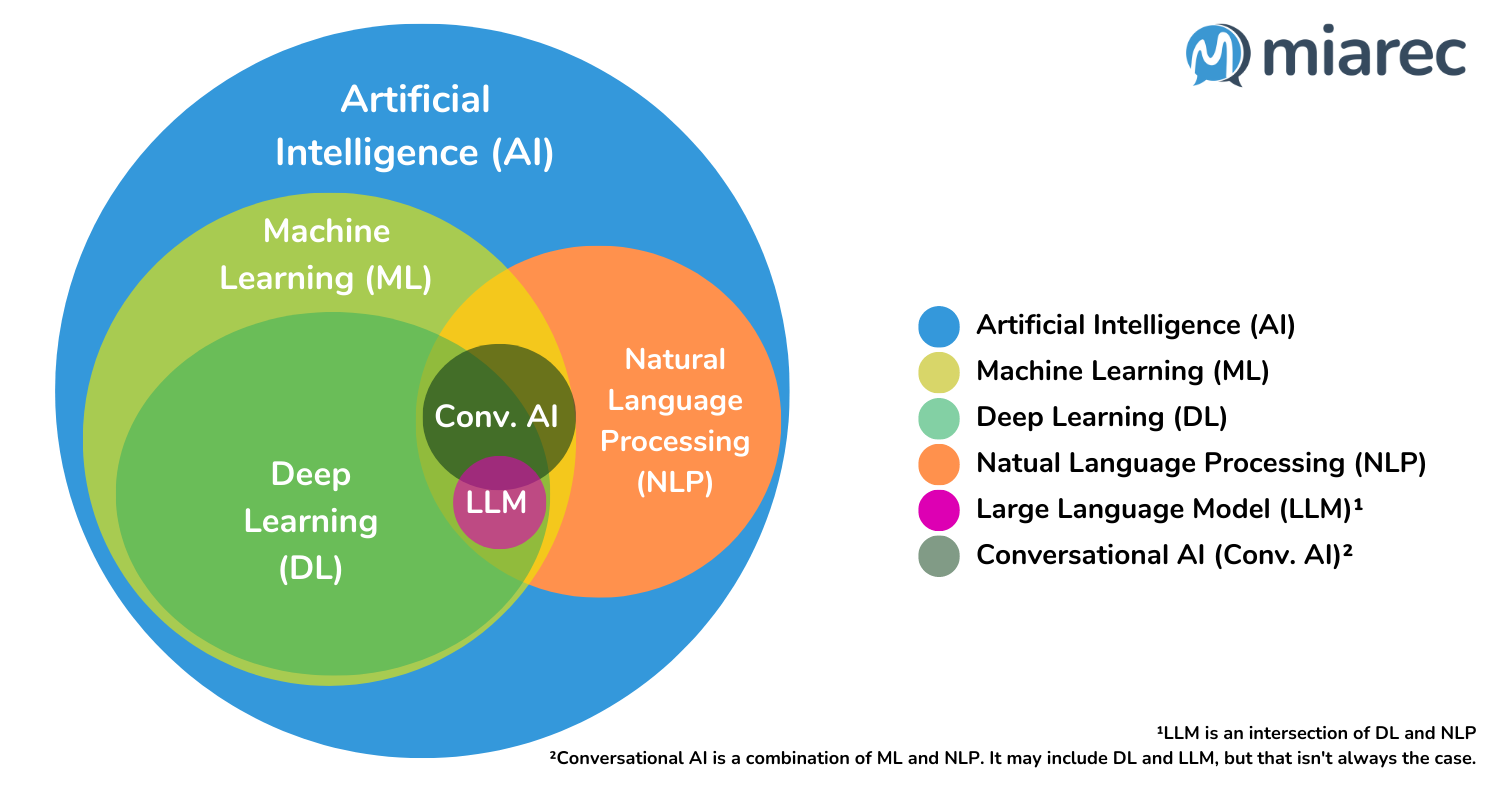
\includegraphics[width=\linewidth]{./figures/genai-relation-diagram.png}
    \caption{Relationship between AI, ML, DL, NLP, and Conversational AI terms. \href{https://blog.miarec.com/contact-centers-ai-definition}{[miarec]}}
\end{figure}\newline
Recent trends in Large Language Models have shown how well they can perform as searching tools or assisting agents. They mimic humanistic thinking and actions by providing chat-like responses to messages. This technology (LLM) can achieve this by its ability to understand the context and flow of conversations; It can recognize whether the prompt is a question, a request to perform an action, or casual natural language tasks like translation and other text modification. Many cloud-based solutions and open-source initiatives have been materialized which has unlocked many possibilities for these models by customizing how they function and augmenting their knowledge.\newpage
These customizations can be summarized in two main points:
\begin{itemize}
    \item Prompt Engineering: This represents how the model is prompted, which has a high impact on the quality of generated responses. There are many techniques related to this; we can precise the context and possibly the history of a chat thread on which the LLM base their answers, specify the tone or length of a response, instruct the model on how it should behave, or provide it with examples on how questions should be answered.
    \item Reinforcement learning from human feedback: For open-source Language Models, one can further train and fine-tune the model. This technique refers to the training of AI model by providing it with direct feedback from humans.
\end{itemize}
\newpage

\section{Retrieval-augmented Generation}
RAG refers to the process of augmenting LLM knowledge by automatically fetching and providing relevant context for the question. It is a technique used to address hallucination and data confinement of generative AI models. This is achieved without re-training the models, which provides a cost-effective approach to improving LLM output so it remains useful and accurate in various scenarios.
\begin{figure}[htbp]
    \centering
    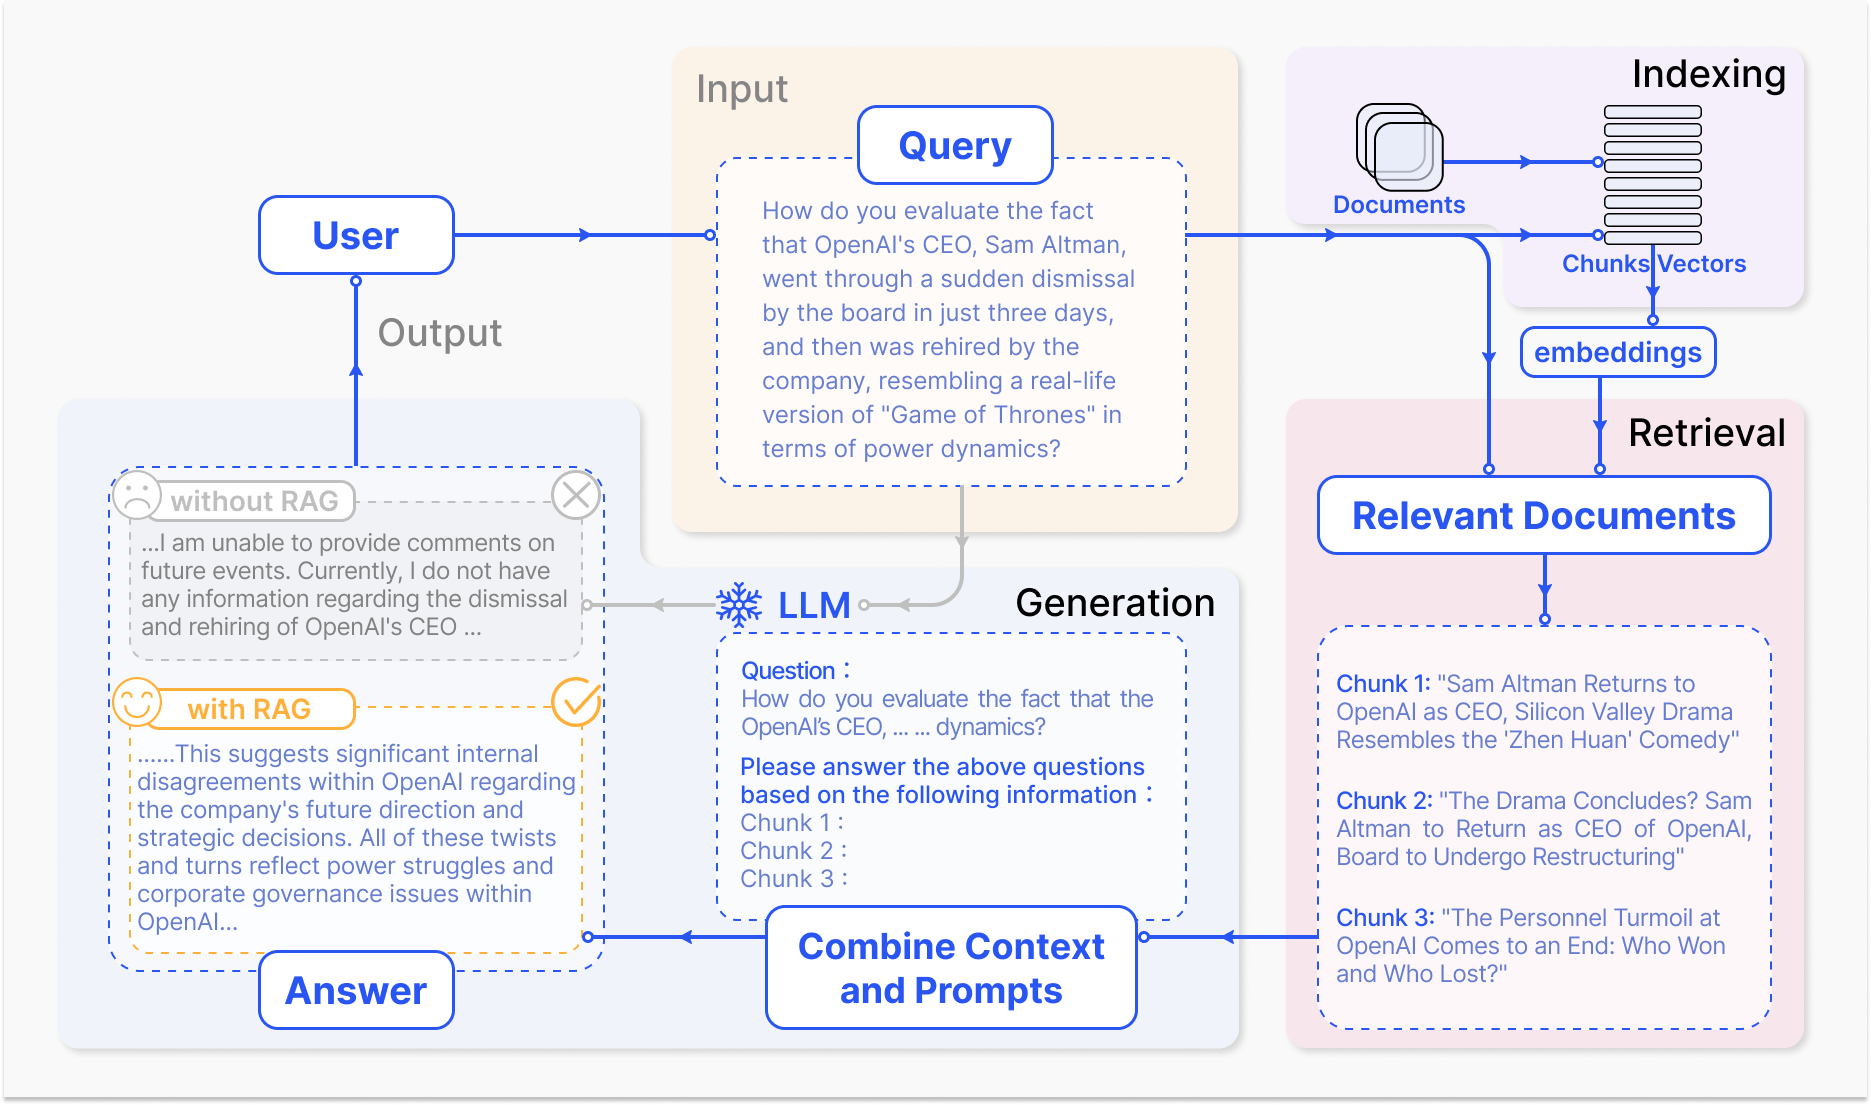
\includegraphics[width=\linewidth]{./figures/RAG_case.png}
    \caption{A representative instance of the RAG process applied to question answering. It mainly consists of 3 steps. 1. Indexing. Documents are split into chunks, encoded into vectors, and stored in a vector database. 2. Retrieval. Retrieve the Top k chunks most relevant to the question based on semantic similarity. 3. Generation. Input the original question and the retrieved chunks together into LLM to generate the final answer. (\href{https://arxiv.org/html/2312.10997v5}{[Retrieval-Augmented Generation for Large Language Models: A Survey]}, March 2024)}
\end{figure}
\newpage

\subsection{Retrieval-augmented Generation paradigms}
Retrieval-augmented Generation process is constantly evolving since the emergence of transformer-based LLMs (GPT models). It has significantly improved on the limitations of LLMs by developing their performance while being cost-effective. Even so, a simple RAG pipeline still exhibit various limitations such as `retrieval-echoing generation` which means outputting the retrieved documents rather than synthesizing answers based on these (which adds more insights to generated text). Moreover, this naive RAG paradigm still introduce hallucinations into answers by confining the generative process to the retrieved documents, which in many cases may not be pertinent to the query (such as in case relevant information not present in the database). In this respect, as more research and engineering is continually being conducted, advanced spinoffs of RAG has emerged to reduce the mis-reckoning and limitations of naive RAG.
\begin{figure}[htbp]
    \centering
    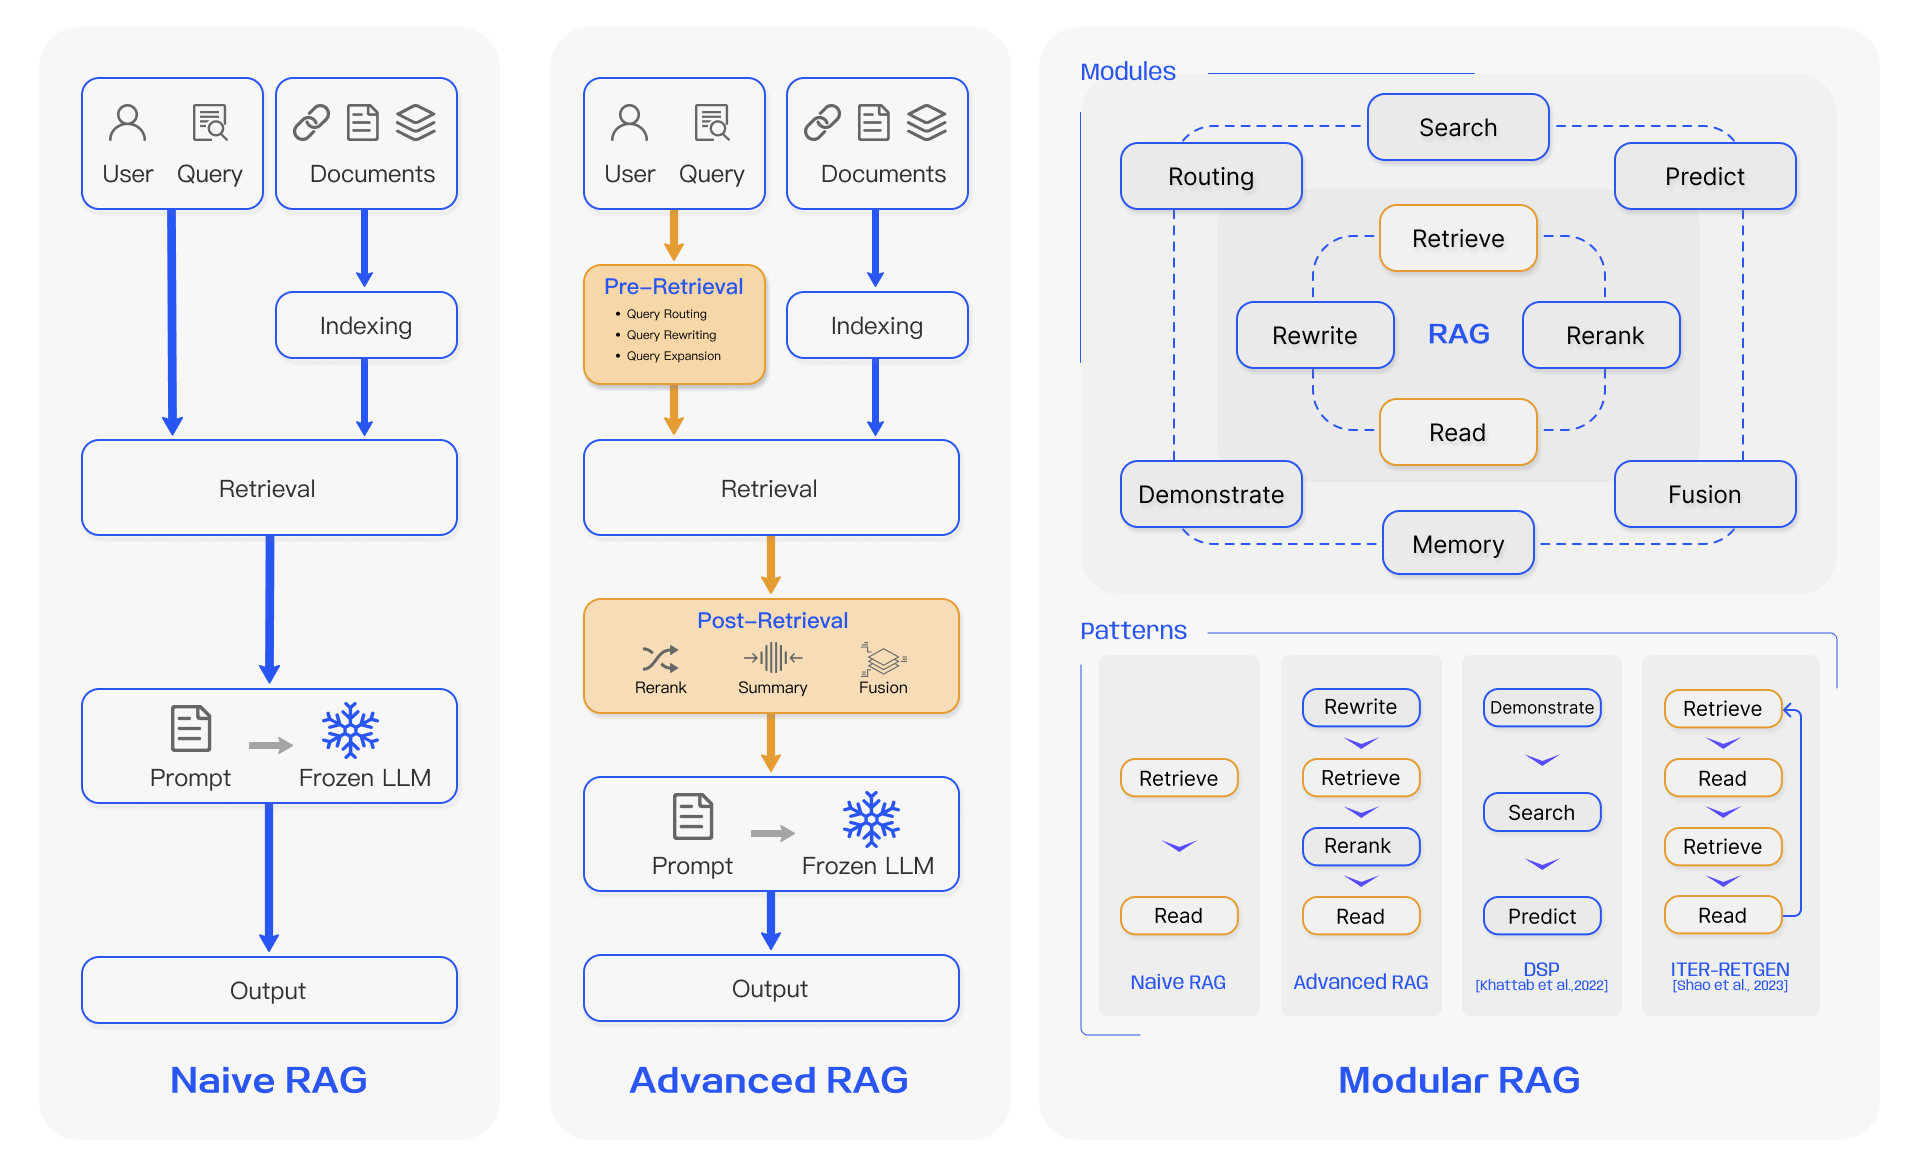
\includegraphics[width=\linewidth]{./figures/RAG_FrameCompre_eng.png}
    \caption{Comparison between the three paradigms of RAG. (Left) Naive RAG mainly consists of three parts: indexing, retrieval and generation. (Middle) Advanced RAG proposes multiple optimization strategies around pre-retrieval and post-retrieval, with a process similar to the Naive RAG, still following a chain-like structure. (Right) Modular RAG inherits and develops from the previous paradigm, showcasing greater flexibility overall. This is evident in the introduction of multiple specific functional modules and the replacement of existing modules. The overall process is not limited to sequential retrieval and generation; it includes methods such as iterative and adaptive retrieval (\href{https://arxiv.org/html/2312.10997v5}{[Retrieval-Augmented Generation for Large Language Models: A Survey]}, March 2024)}
\end{figure}\newpage
In the light of this, we focus on the advanced RAG pipeline structure, which addresses many of the shortcomings of a naive RAG chain without introducing too much complexity to the overall pipeline, (which results in very long question-to-generation delay).
This paradigm involves knowledge base augmentation by routing the input query to other processes and external knowledge sources such as web content, summarization, translation, generative research conducting and LLM instructing through prompt engineering in addition to the re-ranking of retrieval and generation phases' outputs. This is achieved through introducing two additional steps or processes into the overall pipeline: pre-retrieval and post-retrieval. The pre-retrieval phase focuses on obtaining better retrieved results by transforming and interpolating more relevant context into the prompt. The post-retrieval phase focuses on better ranking and incorporating the analyzed context into the prompt. This step (post-retrieval) also addresses content overload by filtering recurrent and repetitive information, compressing or summarizing context, and ranking post-generation output (in our case of multiple LLM selections).\newline
These extra steps would result in better generative AI experience in case knowledge base augmentation is required just-in-time of answer-generation or a re-ranking and compression of either retrieval or generation phase output is required.
\newpage

\subsection{Significance of Retrieval-augmented Generation}
RAG technology can bring many benefits for businesses:
\begin{itemize}
    \item Private and up-to-date data: Even with the high-quality LLM products, it is challenging to maintain relevancy for an enterprise environment. By allowing AI models to connect to external knowledge bases and personal data, much more relevant results can be achieved.
    \item Cost-effective: Even with the availability of open-source LLMs and cloud-based FMs (Foundational Models), the computational and financial costs of re-training such models on domain-specific or private data can be high. By circumventing the re-training phase of LLMs, a huge gain can be brought off using this technique.
    \item More control and customization: It is easy to customize RAG pipelines by developers: Adapting to changing requirements and sources of information, troubleshooting model performance and results, restricting access to some information for authorized users, etc...
    \item User trust: By enabling user choices and interference in the overall process of RAG, users can look up how their choices in information sources and LLM selections affect directly the system results and performance.
\end{itemize}
RAG technique, in many ways, provides an alternative framework to fine-tuning (even though these two techniques are not mutually exclusive) with better adaptability and performance on knowledge-intensive tasks. This is because LLMs struggle to capture new factual information through unsupervised fine-tuning. RAG technique, on the other hand, is designed specifically to control which data is prioritized over another, in addition to instructing the model behavior. By combining these two techniques, we can enhance model capabilities at different levels.\newline
The following figure demonstrates the different optimization methods that affect LLM performance. One can leverage RAG technique for external knowledge augmentation, Fine-Tuning for adapting the model to different domains of expertise, and Prompt Engineering for leveraging LL model's capabilities and functions (e.g. summarization, translation, answering tasks).\newpage
\begin{figure}[htbp]
    \centering
    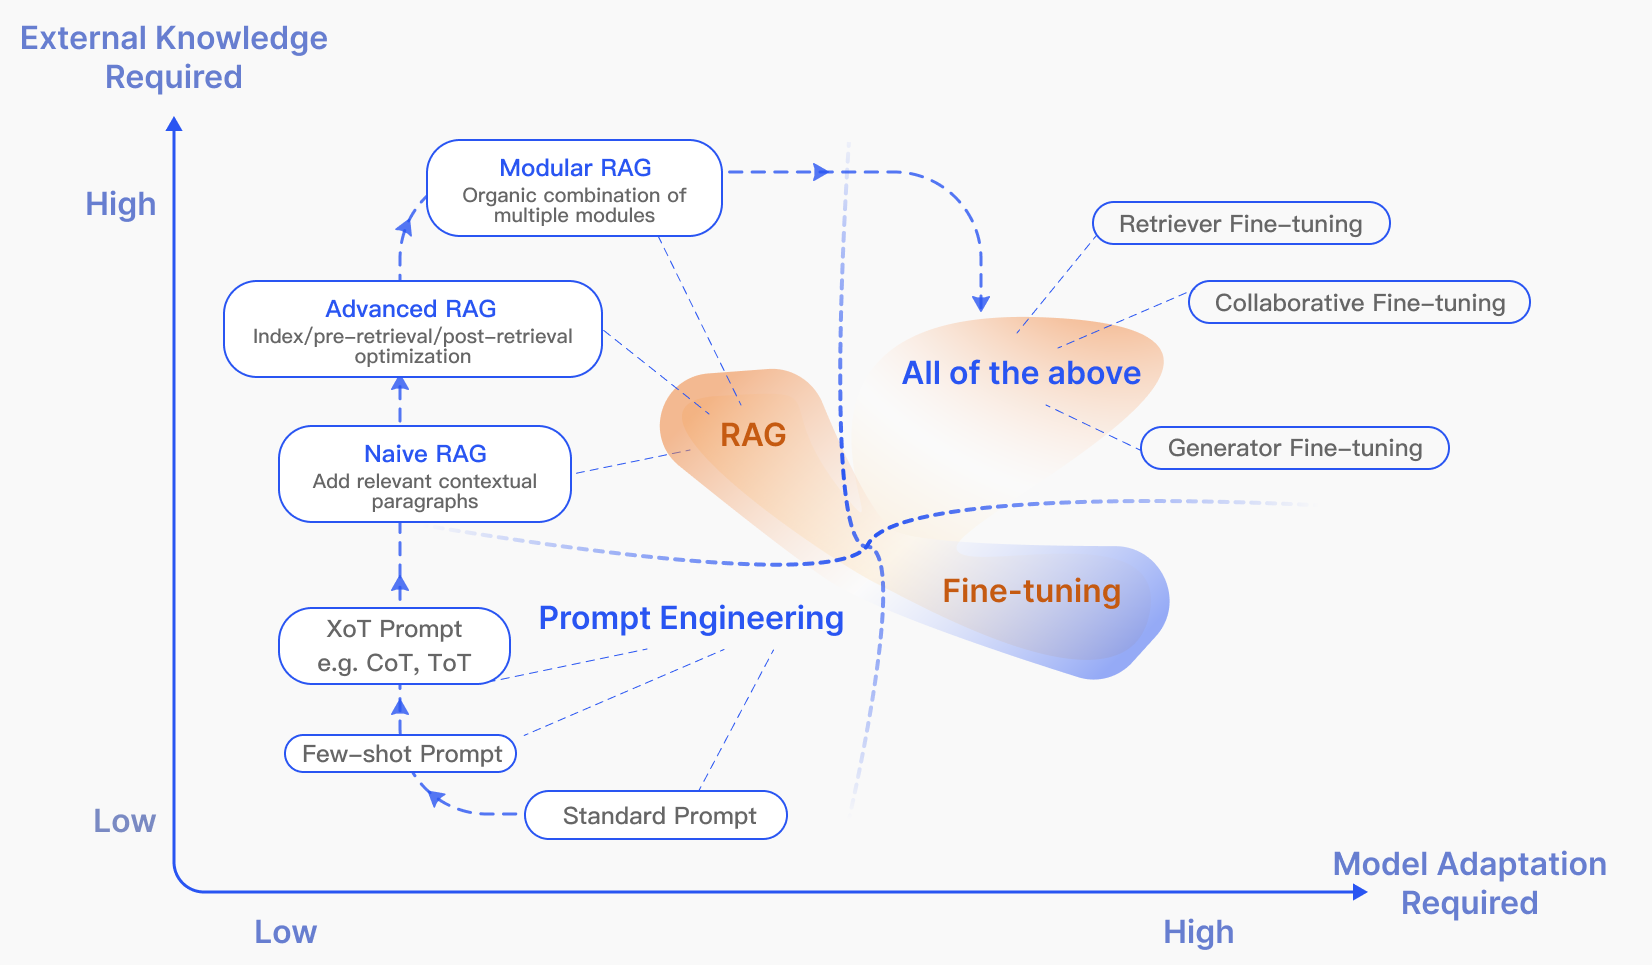
\includegraphics[width=\linewidth]{./figures/rag_FT.png}
    \caption{RAG compared with other model optimization methods in the aspects of “External Knowledge Required” and “Model Adaption Required”. Prompt Engineering requires low modifications to the model and external knowledge, focusing on harnessing the capabilities of LLMs themselves. Fine-tuning, on the other hand, involves further training the model. In the early stages of RAG (Naive RAG), there is a low demand for model modifications. As research progresses, Modular RAG has become more integrated with fine-tuning techniques. (\href{https://arxiv.org/html/2312.10997v5}{[Retrieval-Augmented Generation for Large Language Models: A Survey]}, March 2024)}
\end{figure}
In general, the RAG technique require low model adaptation, rendering it suitable for the interaction with cloud-based LLMs, making the best blend between performance and knowledge augmentation when applied with Prompt Engineering techniques.\newpage
Fine-tuning (or in our case RLHF), on the other hand, can provide LLMs with a reward signal from human feedback to guide them on how to improve their performance in accordance to users' specifications, but this still requires more model adaptability which make it more difficult to implement in different models.
\begin{figure}[htbp]
    \centering
    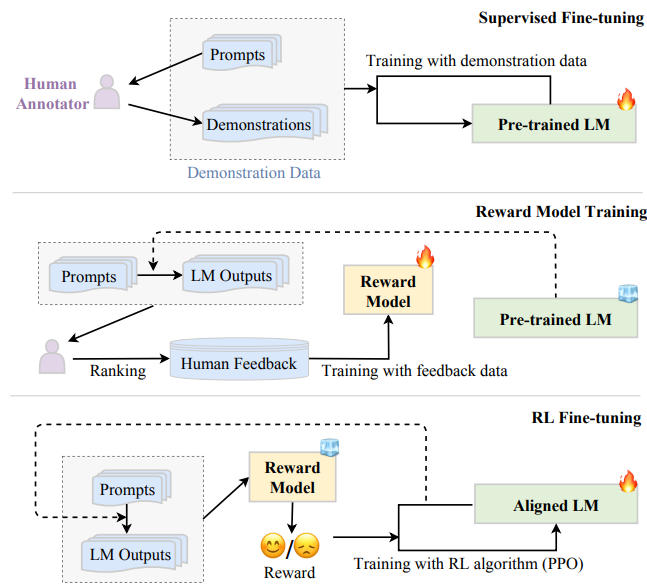
\includegraphics[width=\linewidth]{./figures/rlhf-workflow.png}
    \caption{The workflow of the RLHF algorithm. (\href{https://arxiv.org/pdf/2303.18223}{[A Survey of Large Language Models]}, November 2023)}
\end{figure}
\newpage

\section{Components of a typical RAG pipeline}
The RAG techniques often involves many stages and processes which take place between prompting and answer-generation, as seen in previous sections.
This section introduce high-level (easier to understand) definitions of the discrete components' concepts and their orchestrated functionality.
\newpage

\subsection{Vector Stores}
A vector store refers to a type of database that allows the storage of documents and unstructured data in numerical representations suitable for large volume indexation and retrieval through similarity search algorithms.
\begin{quote}
    "Traditional databases are made up of structured tables containing symbolic information. For example, an image collection would be represented as a table with one row per indexed photo. Each row contains information such as an image identifier and descriptive text. Rows can be linked to entries from other tables as well, such as an image with people in it being linked to a table of names.

    AI tools, like text embedding (word2vec) or convolutional neural network (CNN) descriptors trained with deep learning, generate high-dimensional vectors. These representations are much more powerful and flexible than a fixed symbolic representation, as we’ll explain in this post. Yet traditional databases that can be queried with SQL are not adapted to these new representations. First, the huge inflow of new multimedia items creates billions of vectors. Second, and more importantly, finding similar entries means finding similar high-dimensional vectors, which is inefficient if not impossible with standard query languages."  (\href{https://engineering.fb.com/2017/03/29/data-infrastructure/faiss-a-library-for-efficient-similarity-search/}{[Faiss: A library for efficient similarity search]}, 2017)
\end{quote}
Vector, as in vector store, refers to the embedding vectors of data (arrays of floating-point numbers) which are produced by AI algorithms called embedding models. The output of these models captures the semantics of what is being embedded, which is quite suitable for LLM use cases.\newline
As in LLMs' case, embedding models can be designed specifically to handle textual data or multimedia files. For our case, it is obvious that a suitable embedding model would be the one that best captures the semantics with as little as possible loss of these insightful information.\newpage
\begin{figure}[htbp]
    \centering
    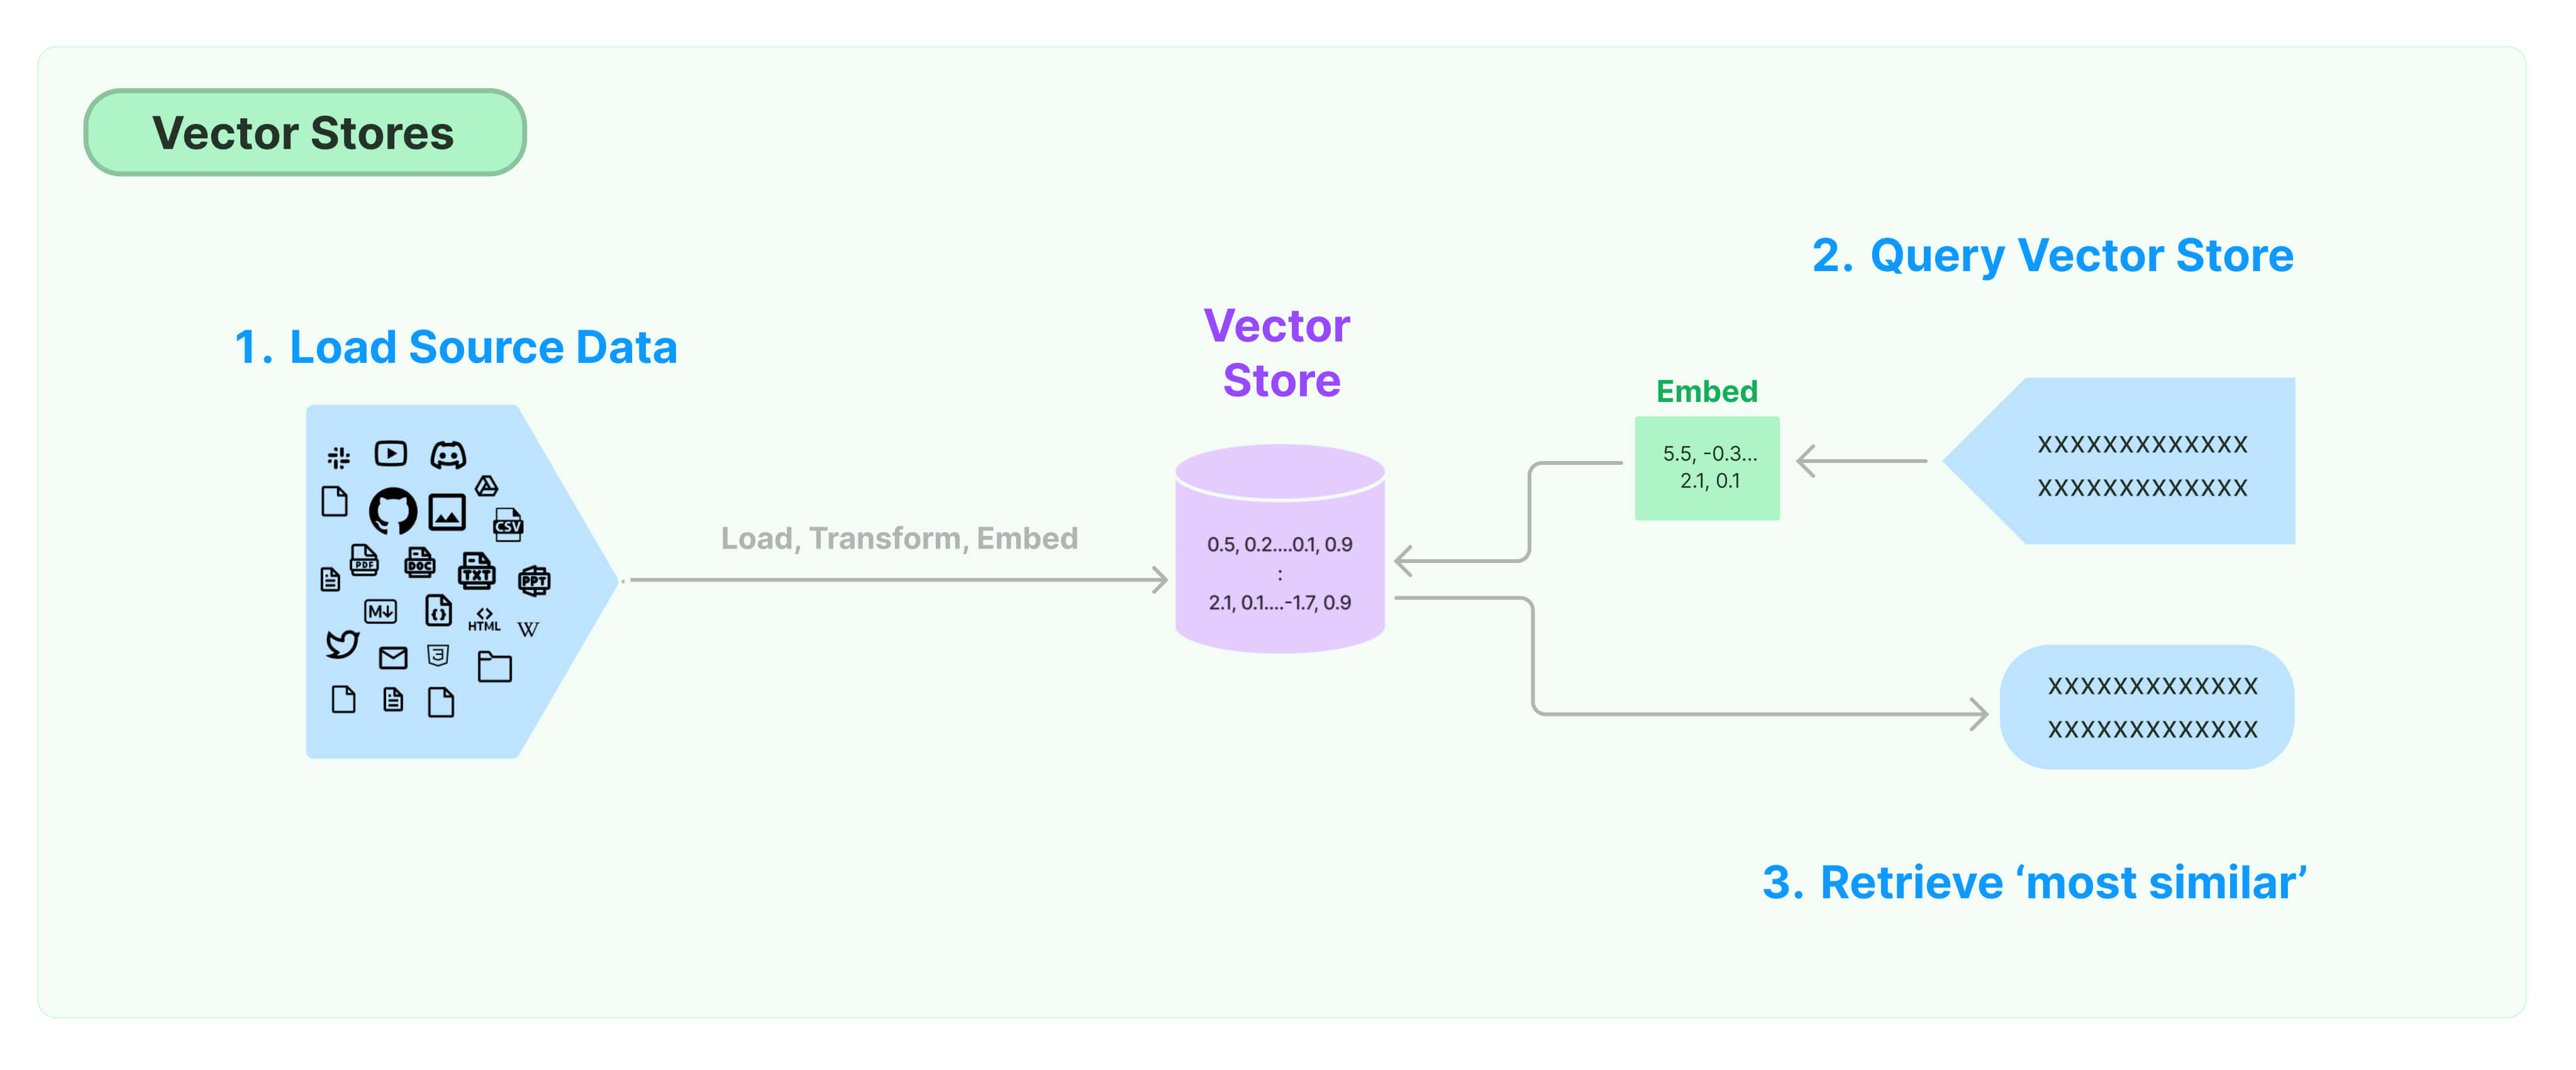
\includegraphics[width=\linewidth]{./figures/vectorstore.jpg}
    \caption{Vector Store Process Diagram. \href{https://python.langchain.com/v0.1/docs/modules/data_connection/vectorstores/}{[LangChain Documentation]}}
\end{figure}
In addition to embedding documents, one should consider the size of these data and the context window limitation of LLMs (each model has some limit on the amount of information it can receive as context). In these conditions, a chunking of documents should be implemented before the embedding and storing phases. This technique allows to divide documents into smaller passages, and marking these with metadata (document id, order etc...) which allow the vector store to structure and store these chunks as they were a single monolithic record. The numerical representations of document sections is adequate to be stored in a vector index in the final phase of indexation.
\begin{figure}[htbp]
    \centering
    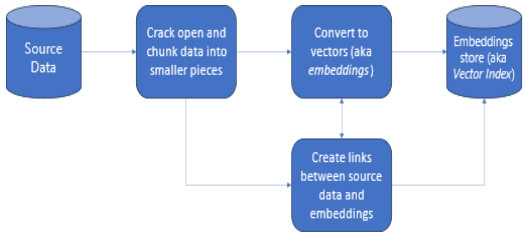
\includegraphics[width=\linewidth]{./figures/chunking-embedding-diagram.png}
    \caption{Embeddings Generation Diagram. (Microsoft, 2023)}
\end{figure}\newline
In addition to the ability to store documents' sections in a suitable form, the vector store index should also be able to search these elements and decode them back into their original textual form. This is achieved through similarity searching algorithms often implemented as constituent functionalities with the vector store. These functions return a number of passages semantically similar to the search term. This is achieved due to the concept of distance calculation between vectors in mathematics.
\begin{figure}[htbp]
    \centering
    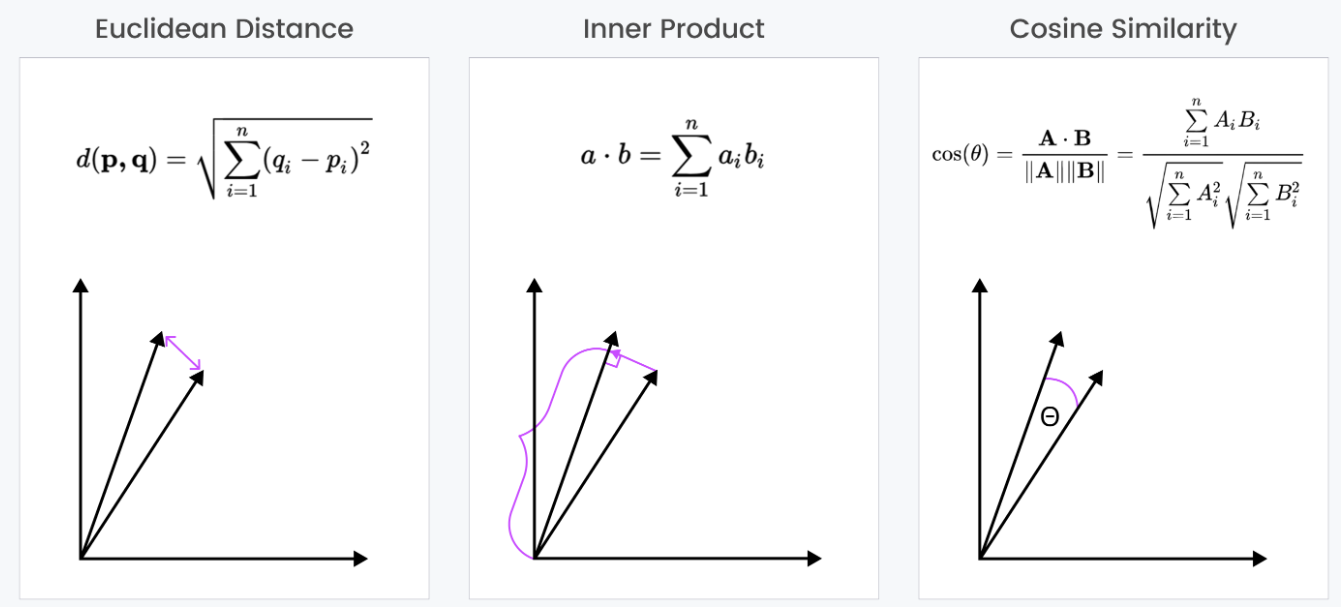
\includegraphics[width=\linewidth]{./figures/vector-distance-metrics.png}
    \caption{Similarity Metrics for Vector Search. \href{https://zilliz.com/blog/similarity-metrics-for-vector-search}{[Zilliz Blog]}}
\end{figure}
\newpage

\subsection{Large Language Model}
The principal component of a RAG system is a textual GAI model which acts as tool that understands user prompts' context and generate textual responses accordingly. Essentially, these models are transformer-based, which allows them to learn complex relationships between words in sentences. For example, a prompt can provide the LLM with context about what kind of text it should generate. The LLM can then use this context to inform its attention mechanism which parts of the prompt it should focus on to generate the most relevant response.
\begin{figure}[htbp]
    \centering
    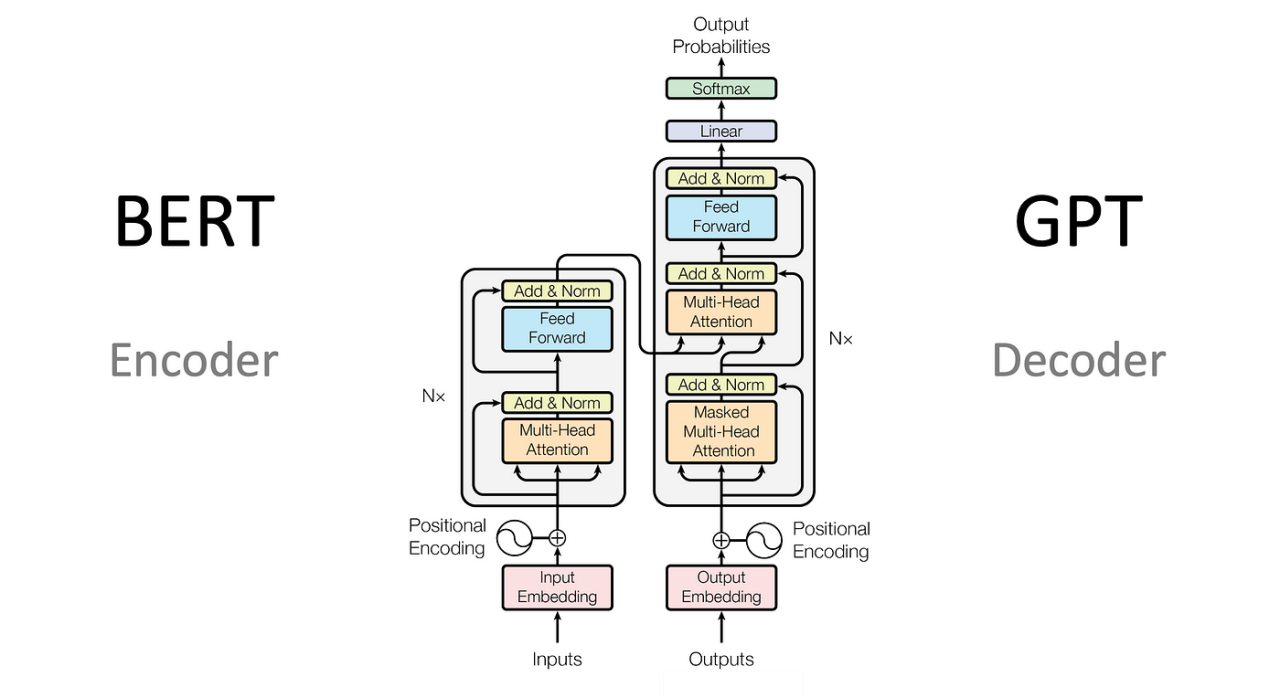
\includegraphics[width=\linewidth]{./figures/The-Transformer-model-architecture.png}
    \caption{An illustration of main components of the transformer model from the original paper, where layer normalization was performed after multiheaded attention. \href{https://arxiv.org/abs/2002.04745}{[On Layer Normalization in the Transformer Architecture (2020)]}}
\end{figure}\newline
The main steps that a transformer-based model pass through are the following:
\begin{itemize}
    \item \textbf{Input Embedding:} The transformer first converts the input text into a series of numerical representations,  which are then passed through a positional encoding layer. This layer adds information about the word’s position in the sentence, which is important because word order matters in a language like English.
    \item \textbf{Encoder Layers:} The core building block of the transformer encoder is the “encoder layer”.  An encoder layer typically consists of two sub-layers: a multi-head attention layer and a feed-forward layer.
    \item \textbf{Multi-Head Attention Layer:} The multi-head attention layer allows the model to attend to different parts of the input sentence simultaneously. This is important for understanding the relationships between words in a sentence.
    \item \textbf{Feed Forward Layer:} The feed-forward layer is a simple neural network that further processes the information from the attention layer.
    \item \textbf{Decoder Layers:} After the encoder has processed the input text, the decoder generates the output text. The decoder also uses encoder layers, but with an additional masked multi-head attention layer. This layer prevents the decoder from attending to future words in the output sentence, which would allow it to “cheat” by looking ahead.
    \item \textbf{Softmax Layer:} The softmax layer converts the decoder’s output into a probability distribution over all the words in its vocabulary. This allows the model to predict the next word in the sentence for instance.
\end{itemize}
\newpage

\subsection{Prompts and Prompt Engineering}
Prompt Engineering (PE) plays a crucial rule in RAG context and LLMs in general. It refers to how the model is prompted, i.e. what does it receive as input. It may include several instructions to the LLM that guides it on how to perform the generation stage. It also can include different parts or steps, such as passing the retrieved context or chat history directly into the prompt, provide it with examples which it should consider when providing answers, or instruct it on how long the answer should be or in which tone it should respond.
\begin{figure}[htbp]
    \centering
    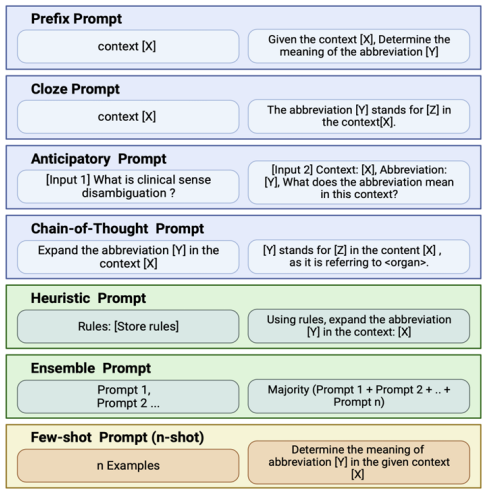
\includegraphics[width=\linewidth]{./figures/prompt-types.png}
    \caption{Types of Prompts: [X]: context, [Y]: Abbreviation, [Z]: Expanded Form
    (\href{https://www.oajaiml.com/uploads/archivepdf/63501191.pdf}{[A Study on the Implementation of Generative AI Services Using an Enterprise Data-Based LLM Application Architecture]}, 2023)}
\end{figure}